\chapter{Experiments}

\section{Classical Computer Vision-based Approach}

\subsection{Glances to Vulnerable Users}
\begin{figure}
    \centering
    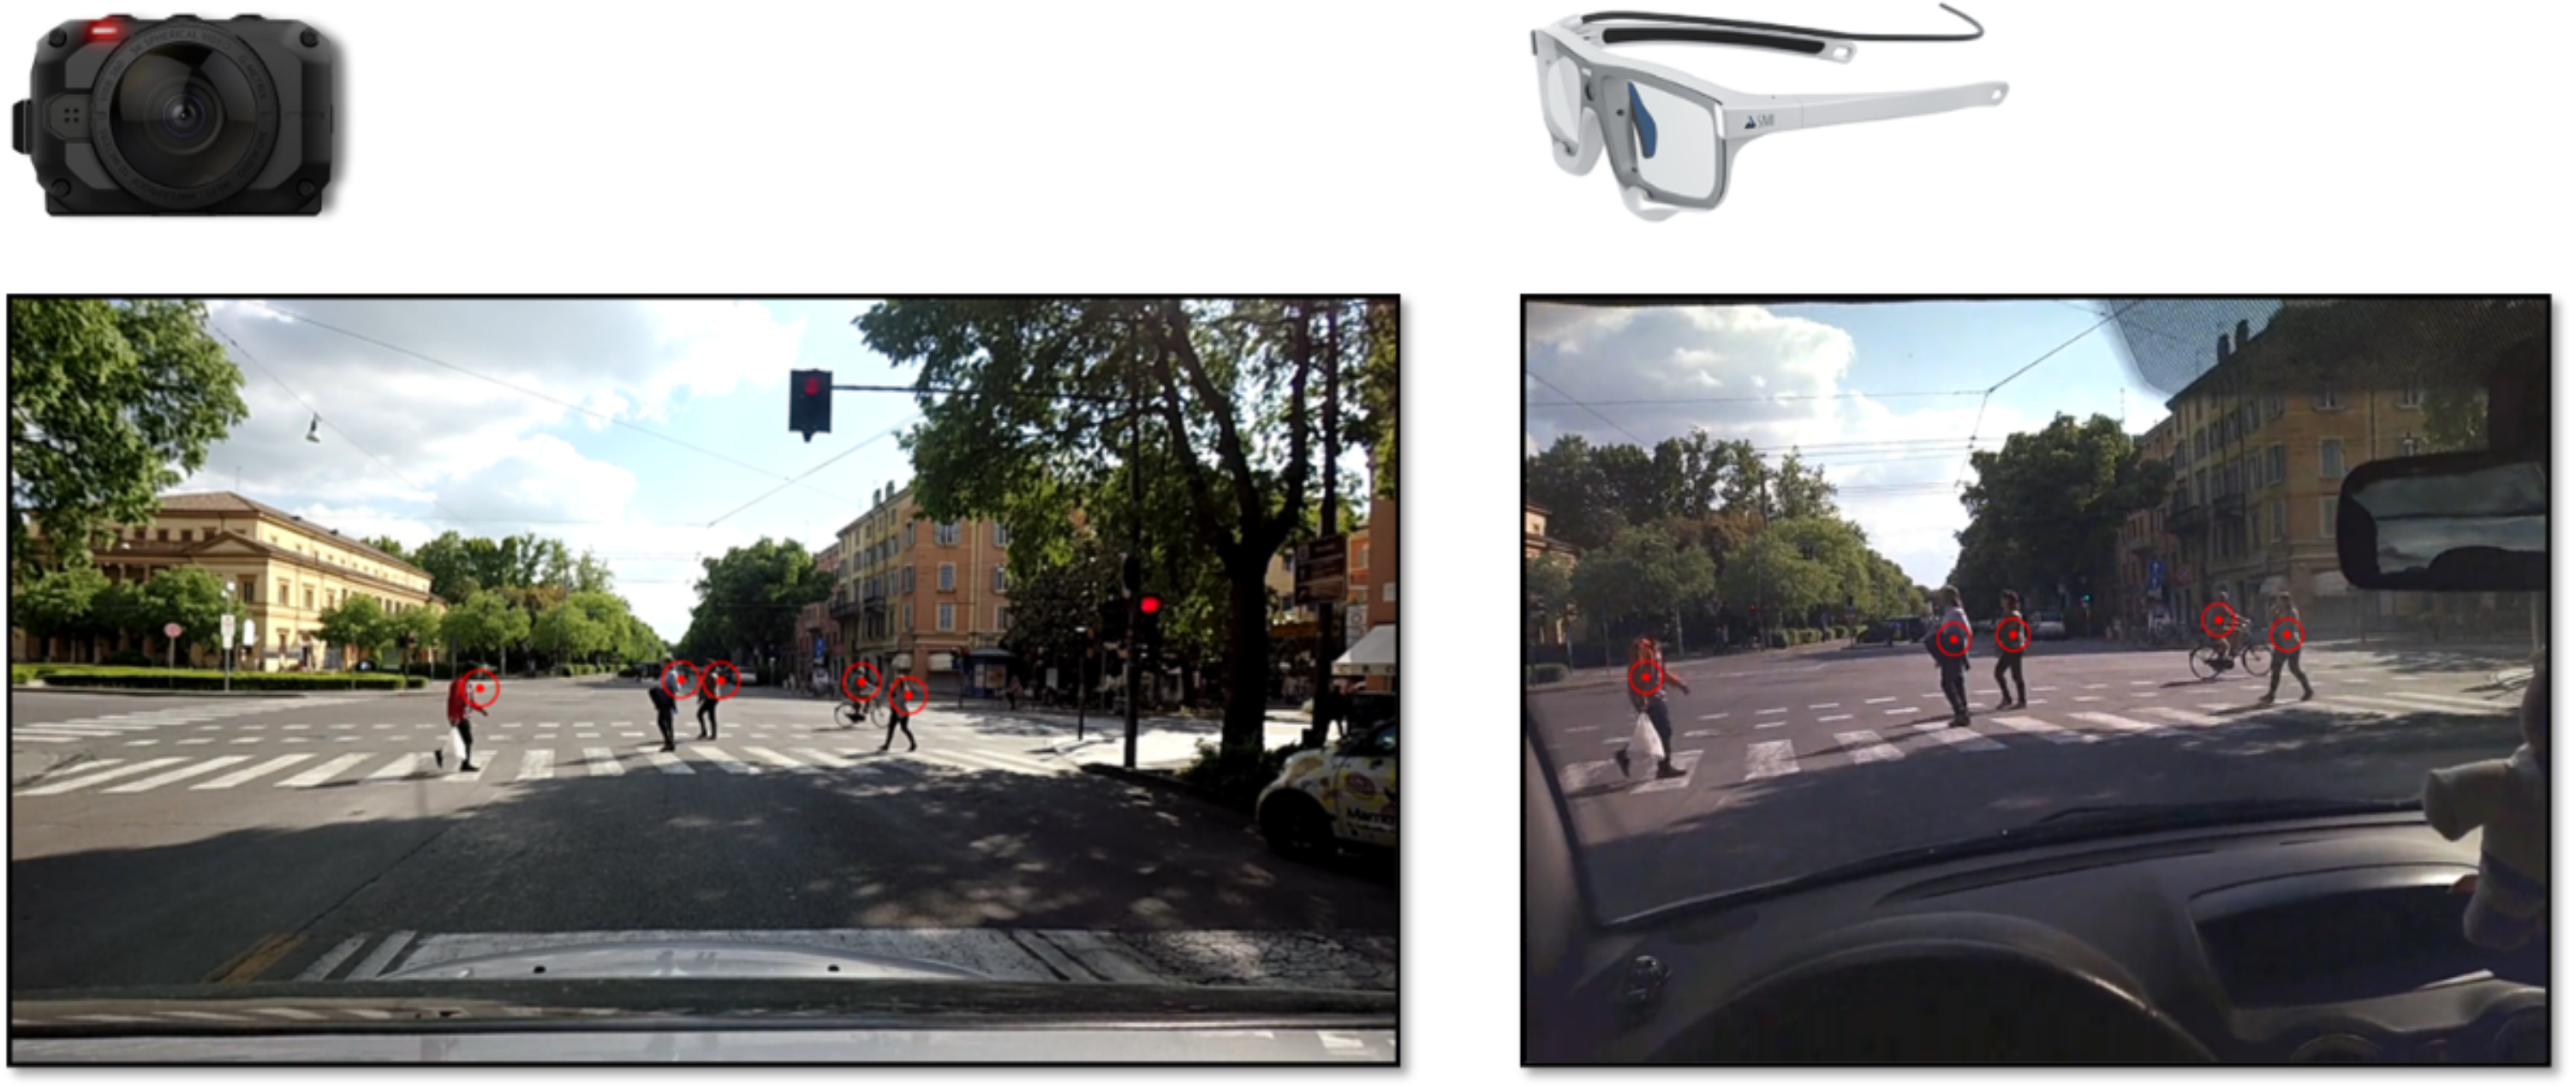
\includegraphics[width=\textwidth]{images/dreyeve/gaze_projection.png}
    \caption{Projection of the gaze from the ETG camera to the RT camera. 
    All the gaze points are manually set.
    \textbf{Left}: Roof top camera view.
    \textbf{Right}: ETG camera view.}
    \label{fig:gaze_projection}
\end{figure}
\begin{figure}
    \centering
    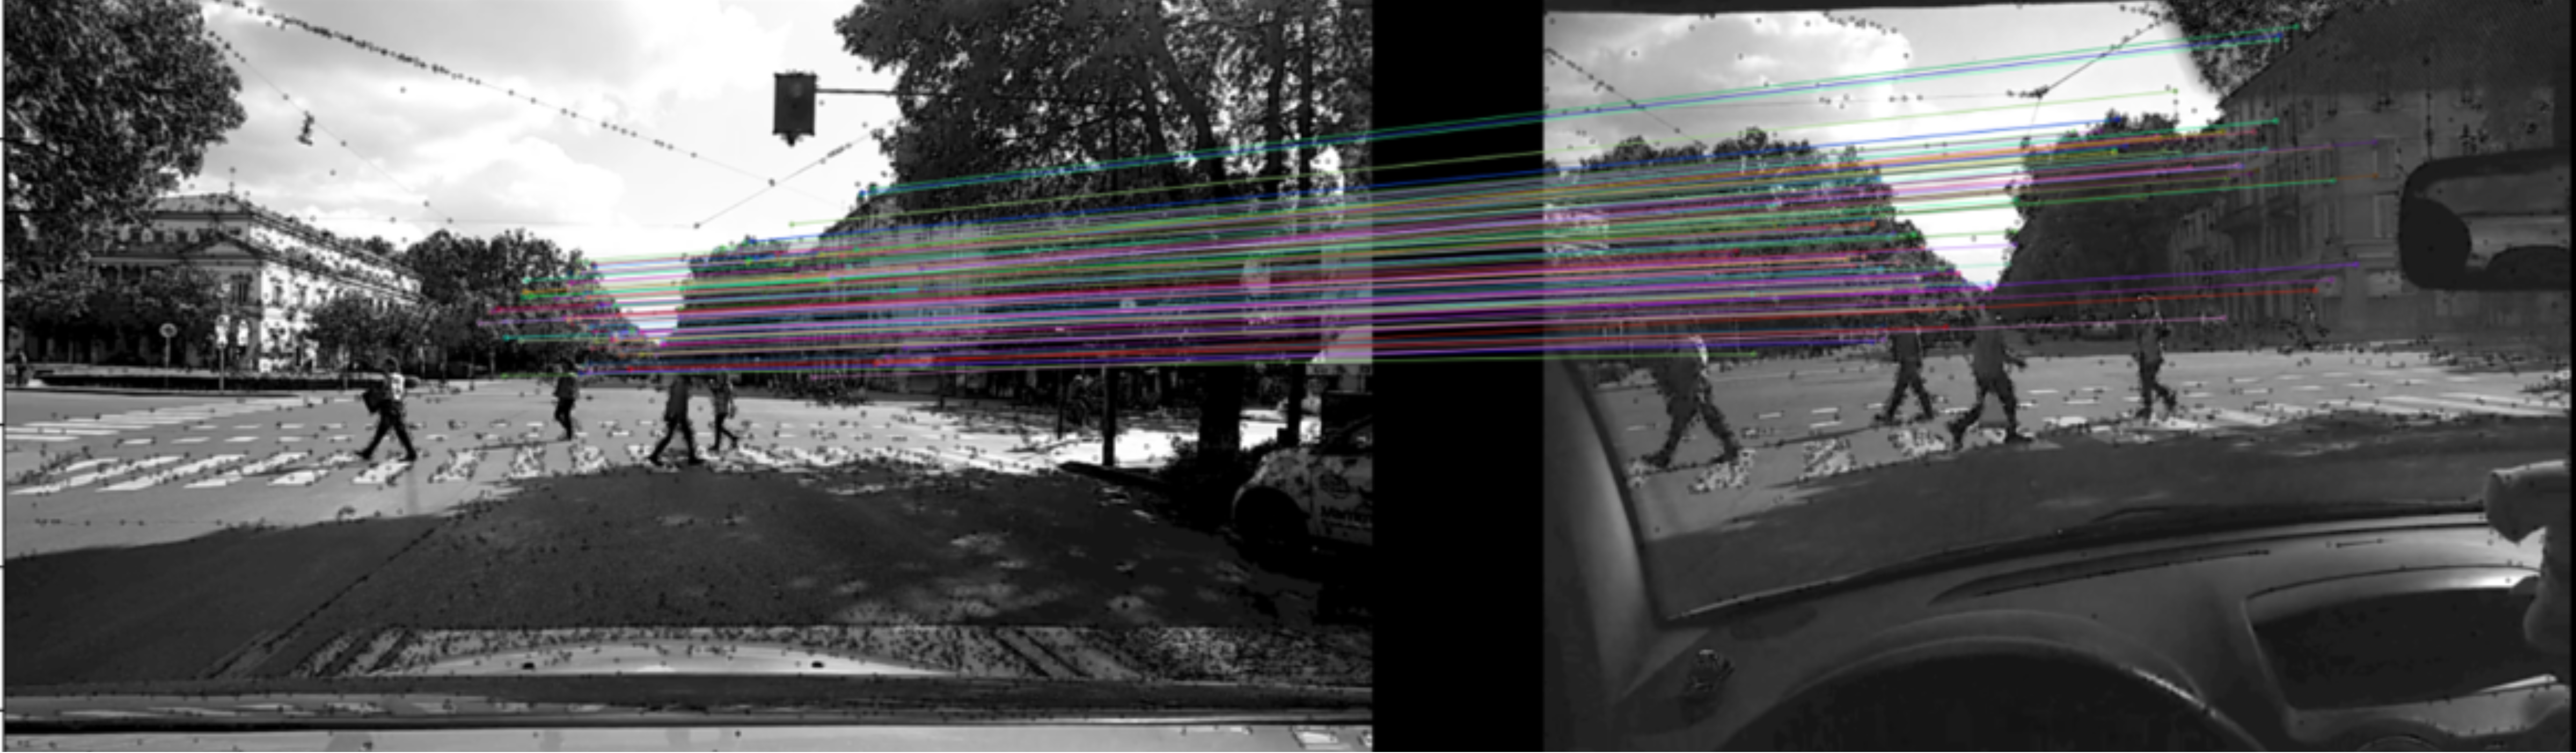
\includegraphics[width=\textwidth]{images/dreyeve/gaze_matchings.png}
    \caption{Projection of the gaze from the ETG camera to the RT camera. 
    All the gaze points are manually set.
    \textbf{Left}: Roof top camera view.
    \textbf{Right}: ETG camera view.}
    \label{fig:gaze_matchings}
\end{figure}
The projection of the gaze from the ETG camera to the RT camera is shown in 
Figure \ref{fig:gaze_projection}. We manually set some gaze points on the 
ETG camera such that they overlap with the vulnerable users. In this way, 
we are setting some operation points that we can use to evaluate the quality 
of the homography estimation. From the figure it is possible to see that the 
projection is not perfect, but it is a good approximation of the gaze in the 
RT camera plane. The small errors are due to the fact that the scene is not 
flat and the homography is a planar transformation. However, most pixels with 
high contrast correspond to objects that are far away from the vehicle, 
therefore the approximation is reasonable.

In Figure \ref{fig:gaze_matchings} we show keypoints' matchings between the 
two images. The keypoints are extracted using the SIFT algorithm.
In a first instance, matchings are computed according to the Lowe's ratio test, 
with a threshold of 0.7. This is to make sure that there is enough Euclidean 
distance from the best matching to the second best matching. Then, we apply 
the RANSAC algorithm, with a threshold of 5 pixels for the reprojection error.
Finally, we compute the homography matrix using the inliers from the RANSAC 
algorithm. To optimize the estimation problem, we set the maximum number of 
iterations to 2000 and a confidence of 99.5\%.

As it is possible to see from Figure \ref{fig:gaze_matchings}, the matchings 
are accurate enough to compute homography. The dark points are all the keypoints 
extracted with SIFT, and the colored lines are the correspondent matchings 
obtained through RANSAC. 
As expected, in a scenario wehre there is a high contrast between the road 
evironment and the sky, the matchings are related to those loactions. 
However, many other keypoints where there is high contrast are detected, for 
example on crosswalks, pedestrians and buildings. They are probably not matched 
beacuse they are not unique enough to satisfy the Lowe's ratio test.

This is a fundamental aspect to consider when designing a system that should be 
used in many different scenarios, during the day and night, in different weather 
conditions, etc. Moreover, in Figure \ref{fig:gaze_projection} and 
\ref{fig:gaze_matchings} we show the results of an especially favorable scenario, 
where there are good conditions of light and contrast, and the driver is looking 
straight ahead.

\subsection{Data Distribution of Dr(eye)ve}
After computing all the projected gaze points, we can focus on the interaction 
of the driver with the vulnerable users. Therefore, it is important to have 
a general overview of the distribution of people in the Dr(eye)ve dataset.
However, considering that the focus is on the interaction \emph{during time},
it is also important to embed poeple's tracking information in the analysis.

Therefore, in Figure \ref{fig:tracking_distribution} we count the number of 
different people that are tracked by the driver. In particular, on the lower 
x-axis there is the total observation time of the person in seconds. On the 
upper x-axis there is the number of frames where the person is tracked, this is 
just to have a different representation of the same data that considers 
preprocessing. On the y-axis there is the number of people observed by the driver 
for the specific amount of time. The distribution is shown in a logarithmic scale 
to better compare the values.
The plots also compare the downtown with all other scenarios. Green bars 
represent the downtown scenarios, while red bars represent the sum of all 
the scenarios in the dataset (therefore including the downtown).

The distribution is right-skewed, with a long tail of people that are observed 
for a short amount of time.
On one hand, this is expected, considering that the driver is usually looking 
straight ahead when driving. On the other hand, it is important to consider 
that some missing data could be due to tracking losses or occlusions with 
ByteTrack, or some non-accurate gaze projections that do not overlap with the 
bounding boxes of the people.

In Figure \ref{fig:tracking_cum_distribution} we show the cumulative distribution 
of the tracking counts. This is a useful representation to understand the number 
of people that are observed, and so tracked, for at least a certain amount of time. 
In this case, the y-axis is linear to better understand the variation of counts 
with respect to the time.

From the cumulative distribution it is possible to see that the total number of 
different observed people is around 110. However, considering a minimum observation 
threshold of 0.3s, which consists of 9 frames, the number of people is reduced 
to 40.
This is a relative small number to consider such a complex interaction betweeen 
humans, in many different scenarios. Moreover, as described in one of the next 
sections, ByteTrack suffers from some tracking losses and mismatching, 
compromising the quality of the data.

It is also important to consider the distribution of recordings with respect to 
time, weather and areas for each driver. In fact the Dr(eye)ve dataset is 
composed of 8 different drivers, each one with a different driving style and 
preferences. In Figure \ref{fig:plot1}, \ref{fig:plot2} and \ref{fig:plot3} we 
show the mentioned plots. Data is enough equally distributed among the drivers, 
with a slight preference for some of them. This means that the behavioral 
information embedded in the dataset can generalize well.

\begin{figure}
    \centering
    \begin{minipage}{0.49\textwidth}
        \centering
        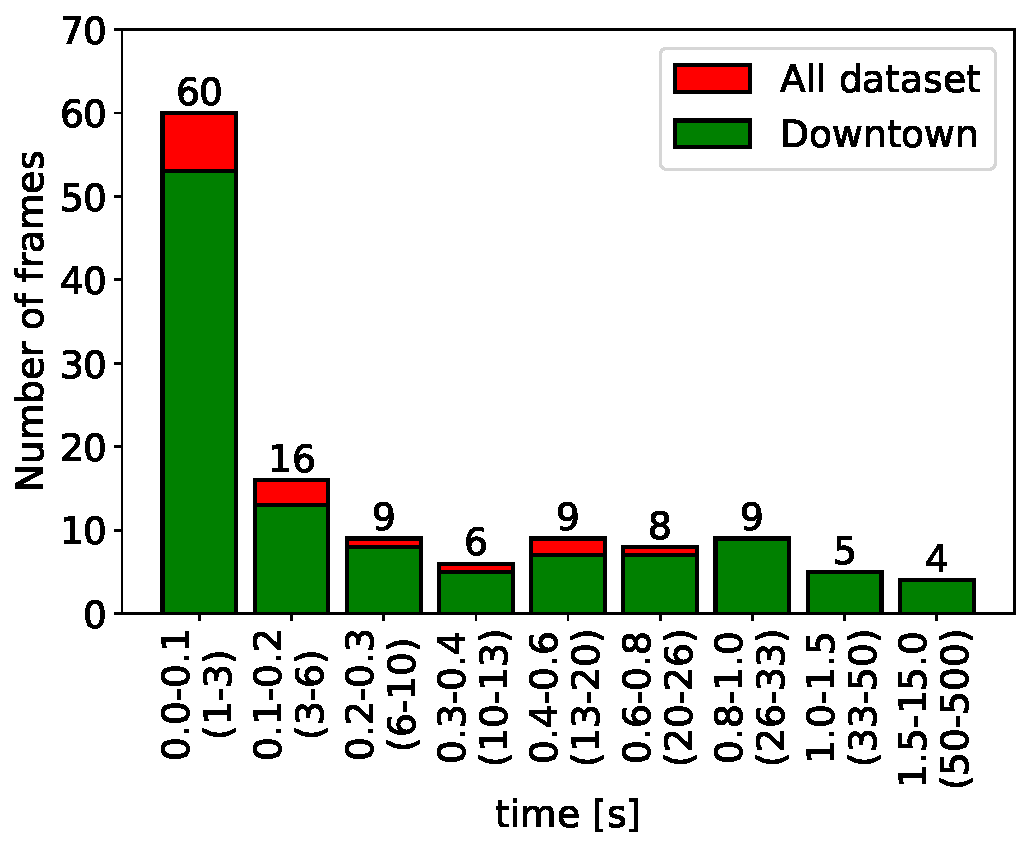
\includegraphics[width=\textwidth]{images/dreyeve/tracking_distrib.pdf}
        \caption{Observation time counts.}
        \label{fig:tracking_distribution}
    \end{minipage}\hfill
    \begin{minipage}{0.49\textwidth}
        \centering
        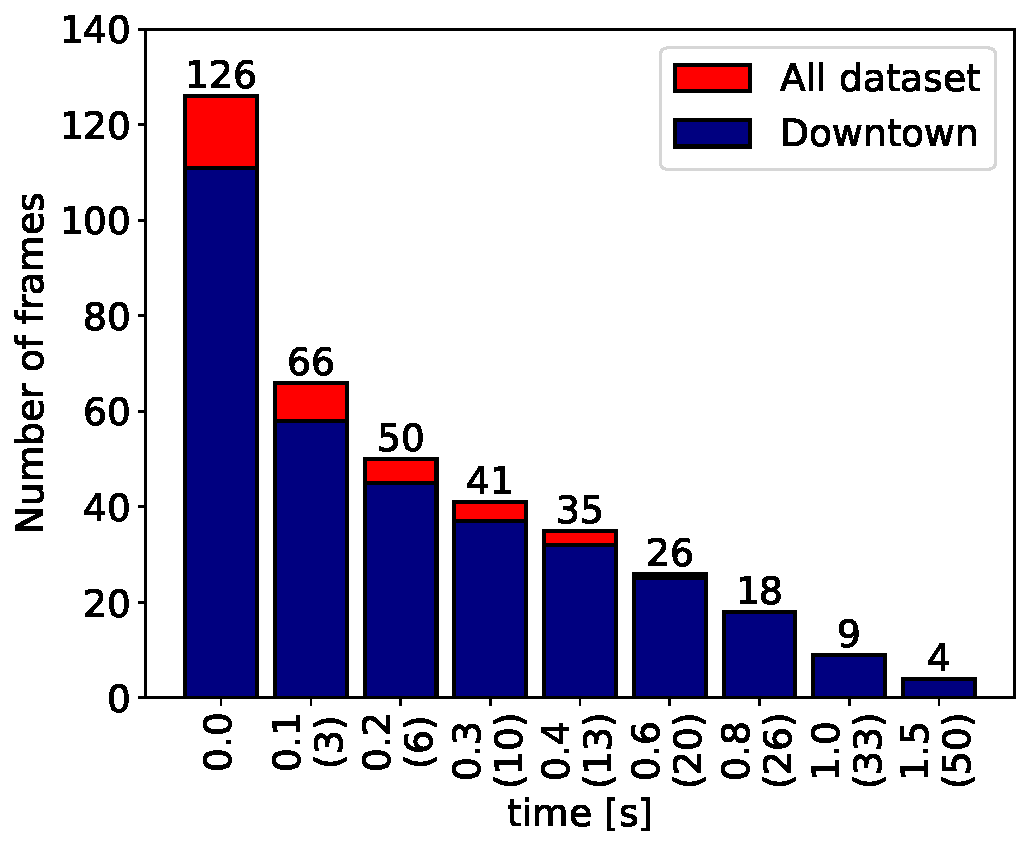
\includegraphics[width=\textwidth]{images/dreyeve/tracking_distrib_cum.pdf}
        \caption{Cumulative of the counts.}
        \label{fig:tracking_cum_distribution}
    \end{minipage}
\end{figure}


\begin{figure}[h]
    \centering
    \begin{minipage}{0.5\textwidth}
        \centering
        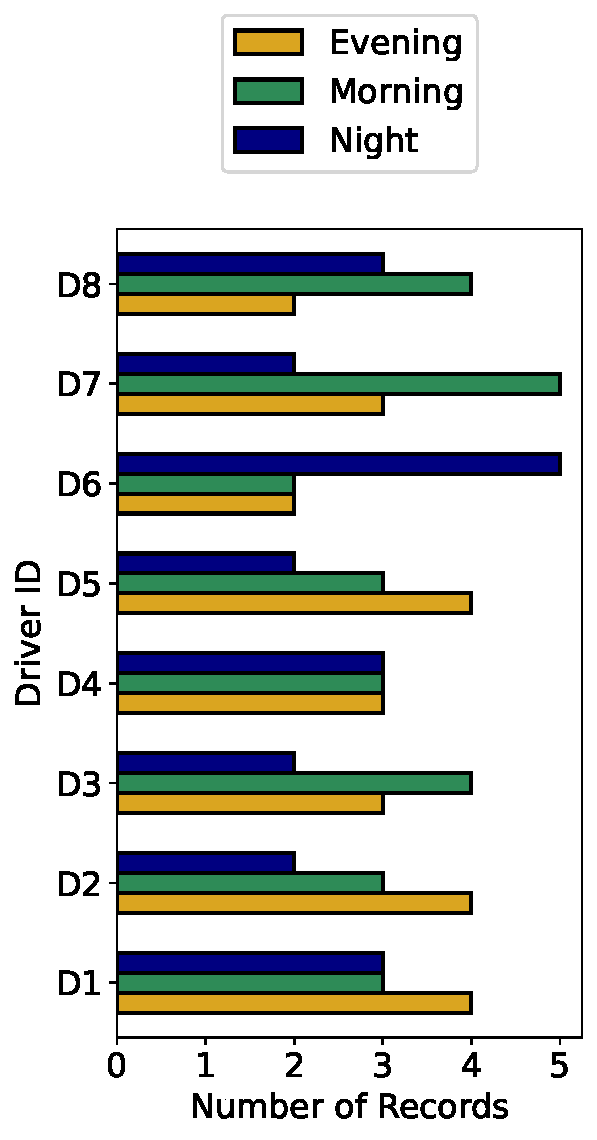
\includegraphics[width=\textwidth]{images/dreyeve/time_distrib.pdf}
        \caption{Distribution of time.}
        \label{fig:plot1}
    \end{minipage}\hfill
    \begin{minipage}{0.5\textwidth}
        \centering
        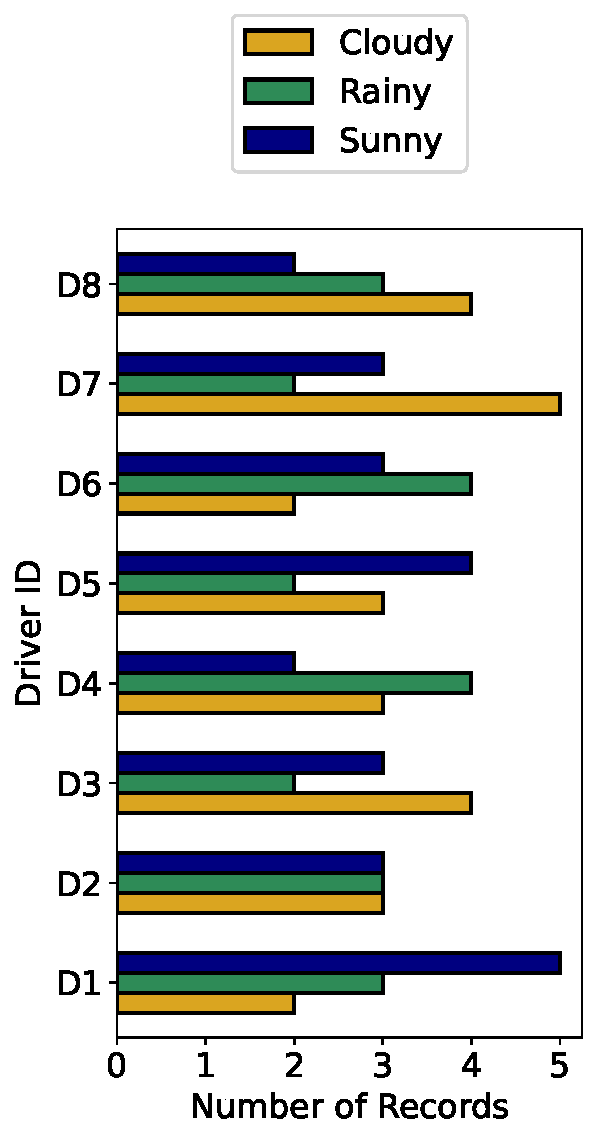
\includegraphics[width=\textwidth]{images/dreyeve/weather_distrib.pdf}
        \caption{Distribution of weather.}
        \label{fig:plot2}
    \end{minipage}\hfill\\\vspace{0.5cm}
    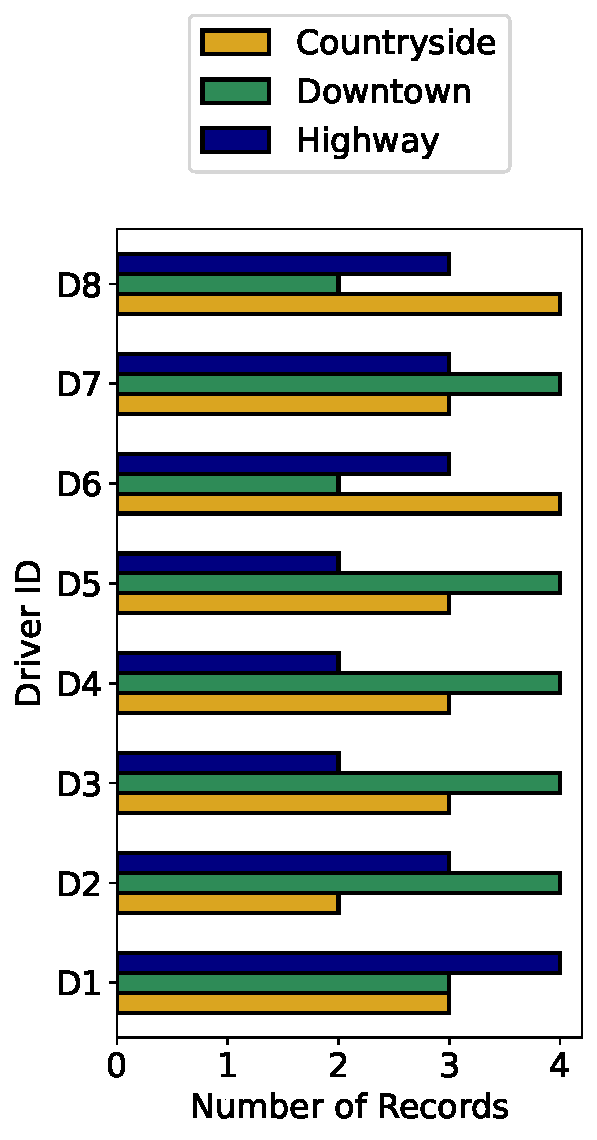
\includegraphics[width=0.5\textwidth]{images/dreyeve/area_distrib.pdf}
    \caption{Distribution of areas.}
    \label{fig:plot3}
\end{figure}

\subsection{Gaze Interaction with Targets}
In Figure \ref{fig:glances} there are six different people that the driver 
observed for at least 0.5 seconds. This minimum threshold is considered a good 
compromise between the time needed to understand the context and the quantity 
of data available, as shown in Figure \ref{fig:tracking_cum_distribution}.
Each plot is referred to a unique person, tracked during the whole sequence.
In particular, it is possible to notice that two different functions overlapped
for each plot:
the observation signal (blue) and the detection signal (red).
Both functions can assume two different states: True or False.

The observation signal is set to True when the driver is looking at the person, 
and False otherwise. The detection signal is set to True when the person is 
correctly detected and tracked by ByteTrack; otherwise it is set to False.
Therefore we can have three different states:
\begin{itemize}
    \addtolength\itemsep{-2mm}
    \item \textbf{D=True, O=True}:\\
    Driver is looking at a visible and detected person.
    \item \textbf{D=True, O=False}:\\
    The person is visible and detected, but the driver is not looking at it.
    \item{\textbf{D=False, O=False}}:\\
    Tracking of person is lost (possible overlapping, occlusion or missed detection).
\end{itemize}
It is important to emphasize that it is not possible to also have the fourth state 
with D=False and O=True, even though the driver could be looking at a person that 
is not detected by ByteTrack at the moment. Therefore, when there are high 
variations of both the observation and detection signals at the same states, 
it is possible that the person is occluded or overlapped, and the driver is 
looking at it. If the frequency is very high, probably the detection algorithm 
is missing some detections between time frames (e.g. there is a variation of 
light conditions, some quick movements, etc.). An example of this case is shown 
in Figure \ref{fig:glances}.d), between 11s and 13s.

Another case is when the person is continuously detected and the driver is looking 
at it only for a short period of time. There can be oscillations of the observation 
during this period, probably due to a small projection error when the case is close 
to some corners of the bounding boxes. This can be amplified in quick movements' 
scenarios. An example of this case is shown in all the figures in different 
periods of time.

If the person is detected continuously and the observation signal varies slowly 
and periodically, like in Figure \ref{fig:glances}.b-e), it is possible that the 
driver is looking at different parts of the scene keeping updating the attention 
towards them.

Finally, in Figure \ref{fig:glances}.c-f) there are some cases where the person 
is not glanced at by the driver, and the detection signal varies at high 
frequency. This is the case when the person is visible and tracked, but the driver 
is not paying attention to it. 

This is a good example of the importance of contextualizing the scene through 
perception and driver's data. However, there are many complex cases that are 
difficult to explain with just these two signals, especially when it is 
fundamental to consider possible tracking losses or mismatchings.

\begin{figure}
    \raggedright
    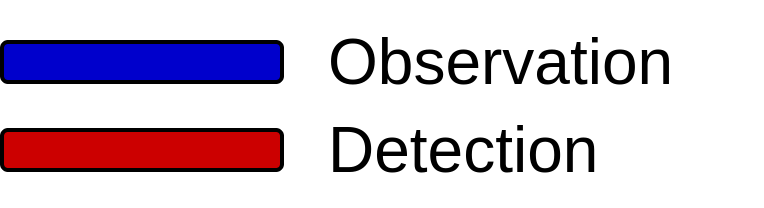
\includegraphics[width=0.23\textwidth]{images/dreyeve/gazes/glances_legend.png}\\
    \centering
    \begin{minipage}{0.5\textwidth}
        \centering
        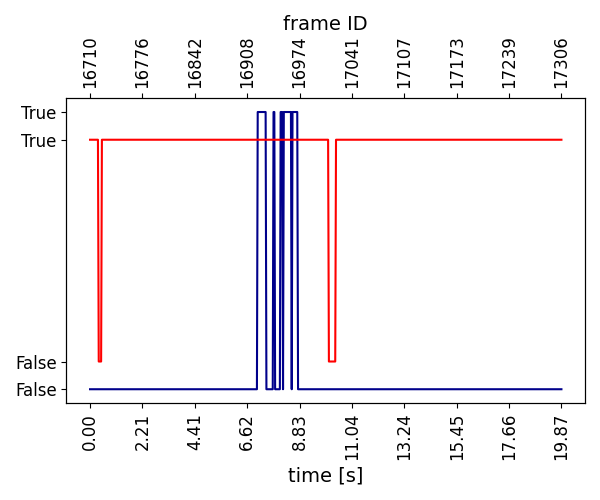
\includegraphics[width=\textwidth]{images/dreyeve/gazes/1.png}
        \textbf{a)}
    \end{minipage}\hfill
    \begin{minipage}{0.5\textwidth}
        \centering
        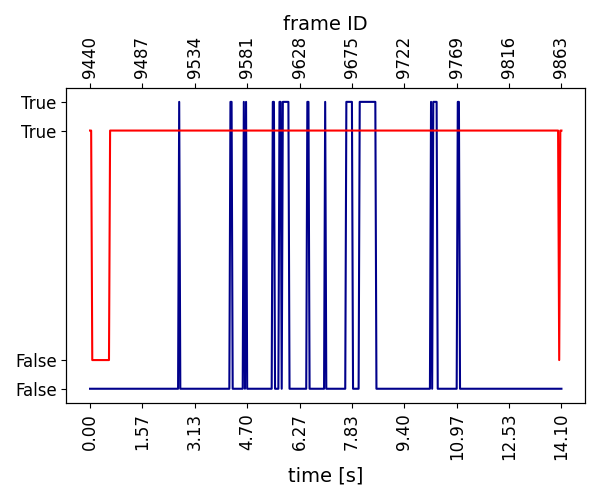
\includegraphics[width=\textwidth]{images/dreyeve/gazes/2.png}
        \textbf{b)}
    \end{minipage}\hfill \\\vspace{0.2cm}
    \begin{minipage}{0.5\textwidth}
        \centering
        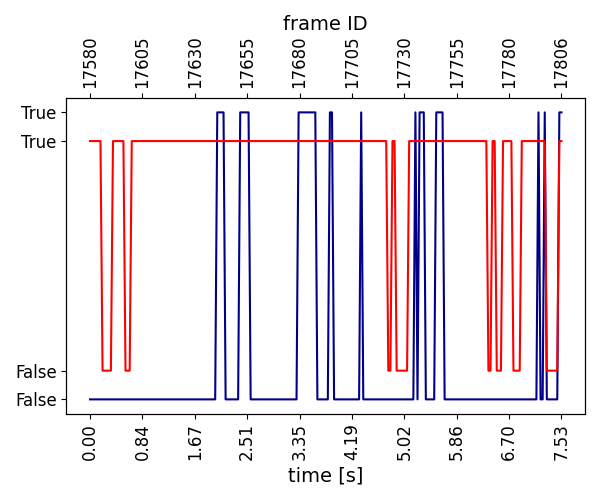
\includegraphics[width=\textwidth]{images/dreyeve/gazes/3.png}
        \textbf{c)}
    \end{minipage}\hfill
    \begin{minipage}{0.5\textwidth}
        \centering
        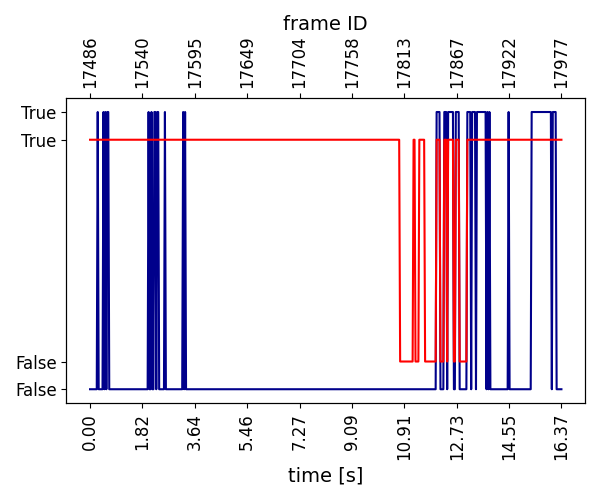
\includegraphics[width=\textwidth]{images/dreyeve/gazes/4.png}
        \textbf{d)}
    \end{minipage}\hfill\\\vspace{0.2cm}
    \begin{minipage}{0.5\textwidth}
        \centering
        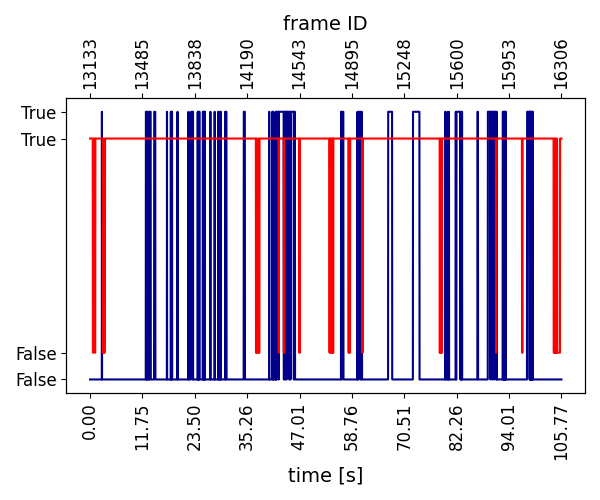
\includegraphics[width=\textwidth]{images/dreyeve/gazes/5.png}
        \textbf{e)}
    \end{minipage}\hfill
    \begin{minipage}{0.5\textwidth}
        \centering
        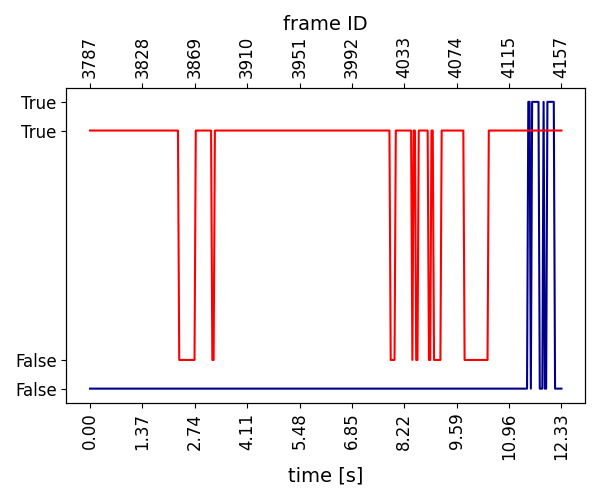
\includegraphics[width=\textwidth]{images/dreyeve/gazes/6.png}
        \textbf{f)}
    \end{minipage}
    \caption{Driver glances towards people in the Dr(eye)ve dataset 
    (minimum glance threshold is set to 0.5s).}
    \label{fig:glances}
\end{figure}

\subsection{Tracking Performance}
As mentioned before, analyzing driving interatctions between the driver and 
vulnerable users is a complex task that can be compromised by tracking errors.
Even though ByteTrack is a state-of-the-art tracking algorithm, especially 
designed for scenarios with occlusions and overlapping, it can still suffer 
from some mismatches and tracking losses.
It is complicated to find out when the tracking is lost, from the output of 
the algorithm. Even worse, if there is a tracking mismatch, driver's gaze 
information can be compromised, leading to wrong conclusions about the interaction 
between the driver and the other targets.

In Figure \ref{fig:tracking_mismatch} we show some examples of tracking mismatches
in a driving scenario of Dr(eye)ve.
In particular, four different frames from the roof top camera are shown. 
We decided to show the frames where there are overlapping or occluded people, 
to emphasize the complexity of the tracking task.

From Figure \ref{fig:tracking_mismatch}.a) to Figure \ref{fig:tracking_mismatch}.b)
the tracked person (with ID 342) overlaps with another person that is walking on 
the crosswalks. In this case the tracking is not lost, and the person is correctly 
tracked.

From Figure \ref{fig:tracking_mismatch}.b) to Figure \ref{fig:tracking_mismatch}.c)
the same tracked person overlaps with another target, but this time there is 
a tracking mismatch. The bounding box is now assigned to the incoming person, 
and the tracked person is lost.

A similar case is shown from Figure \ref{fig:tracking_mismatch}.c) to 
Figure \ref{fig:tracking_mismatch}.d). The tracked person is mismatched with 
another incoming person.

Even though lighting conditions are optimal, and people are not occluded by 
other objects, tracking mismatches can still happen. This is a fundamental 
aspect to consider when designing a feature for an ADAS system. 
Another aspect is that, despite the presence of other objects in the background 
like cars, the tracking algorithm is able to correctly keep the right tracking, 
considering that the backbone model is not specifically trained on detecting 
people in driving scenarios. This is a good sign of the robustness of the 
algorithm with respect to the background environment, and could be enhanced 
through an ad-hoc fine-tuning of the detection stage on driving scenarios.
\begin{figure}
\centering
\includegraphics[width=0.85\textwidth]{images/dreyeve/tracking_mismatch.png}
\vspace{0.4cm}
\caption{ByteTrack's tracking mismatches in a driving scenario.}
\label{fig:tracking_mismatch}
\end{figure}

\subsection{Monocular Depth Estimation with MiDaS}
In this section we show and evaluate the results of the monocular depth estimation 
computed by MiDaS \cite{midas}. To evaluate the quality of the estimation it 
is necessary to have a ground-truth information to compare with. In this case, 
Dr(eye)ve dataset does not provide any depth information by default, because no 
depth sensors are used. 
Therefore, the idea is to validate the model on another 
dataset that provides depth information and a good variety of scenarios, from 
downtowns to highways, with different weather conditions, etc. 
We decided to use the NuScenes dataset \cite{nuscenes}, that provides both 
LiDAR and camera data.

In Figure \ref{fig:mde} we show the results of the monocular depth estimation 
for an entire scene of the NuScenes dataset. The left image is an heatmap of 
the relative inverse depth estimated by MiDaS, and compared with the ground-truth 
pointclouds taken from the front LiDAR. In particular, it is necessary to mention 
that MiDaS provides a \emph{relative} inverse depth that depends on the specific 
image, depending on the distance of closer and farther objects.
Considering that the comparison is not straightforward for the entire dataset, 
we decided to show the results for one entire scene, where at least the same 
environment is present in all the frames. Then the relative inverse depth is 
normalized to be in the range $[0, 1]$, and compared with the absolute depth 
of correspondent points in the LiDAR pointcloud. This means that non-correspondent 
pixels in the dense depth map are masked out.
Finally, we decided to use an heatmap to not only show the distribution of points, 
but also find how frequently the model makes some errors in the estimation.
Considering the preprocessing of the data, a reference curve is also shown. 
It spans from 4m to 60m on the x-axis and from the 
minimum to the maximum of the relative inverse depth on the y-axis. This is to have 
a unique function that is able to map all values in the two domains.
To be precise, the reference curve should not span only up to the maximum 
value of the pointcloud, but it should consider the maximum distance in the 
entire scene. However, this is a good approximation to have a general idea 
of the quality of the estimation, leveraging ground-truth data. In fact, 
from the experiments we realized that the model is more accurate in estimating 
high relative distances between objects in the scene, and this is usually related 
to closer-to-the-ego-vehicle objects. Moreover, LiDAR pointclouds can reach 
up to 100m, but the further points are, the more sparcely they are distributed
in the 3D space.

Another important aspect to consider is the output of MiDaS, that is the relative 
inverse depth. This means that the closer the object is, the higher the output 
of the model is. This is the opposite of the LiDAR pointcloud, where the closer 
the object is, the lower the depth value is. However, we decided not to invert 
one of the two signals to have a better comparison at closer distances, but also 
including farther estimations, with the output tending to zero for the farther objects.

From the results in the heatmap it is possible to notice that the model is able 
to estimate the depth of closer objects with a good approximation, but it is 
much less accurate for farther objects. Regarding closer objects, there 
are many point clouds related to the road that, considering its shapes, it is 
probably easier to estimate. On the other hand, farther objects are usually 
less visible in the image, and the model is not able to estimate them correctly. 
Moreover, there are some close pointclouds that are estimated far from the ego-vehicle,
and it adds a consistent error for the evaluation.

Considering the problems to evaluate the accuracy of the model with respect to 
the ground-truth data, we decided to report two error metrics: the root mean 
squared error (RMSE) and the relative root mean squared error (RRMSE). 
They are calculated as follows:
\begin{align}
    \text{RMSE} = \sqrt{\frac{1}{n} \sum_{i=1}^{n} \left(d_i - \hat{d}_i\right)^2} \qquad\qquad
    \text{RRMSE} = \sqrt{\frac{1}{n} \frac{\sum_{i=1}^{n}{\left(d_i - \hat{d}_i\right)^2}}{\sum_{i=1}^{n}d_i^2}} \nonumber
\end{align}
where $d_i$ is the normalized depth of the i-th point in the LiDAR pointcloud, 
and $\hat{d}_i$ is the relative depth estimated by MiDaS. In total 
there are $n$ point clouds visible in the scene. As it possible to notice from the 
definition of the metrics, the RRMSE is a normalized version of the RMSE with 
respect to the average depth of the scene. This is useful to understand the 
quality of the estimation in all the dataset. However, we have inverted the 
relative depth obtained from MiDaS, therefore small values in the dense depth 
map heavily affect the RRMSE.

The right image, on the other hand, 
shows the projection of the LiDAR pointcloud on the image plane, through the 
camera calibration matrix. Each point is colored according to the depth value 
in the LiDAR pointcloud. This is to have a visual understanding of the distribution 
of pointclouds in one frame of the scene. As shown in the picture, the scenario 
corresponds to a downtown environment, with many buildings and cars. 
Closer point clouds can be related to the road, parked vehicles on the sides, 
road obstacles, etc. Farther point clouds are usually related to buildings, 
trees, and other objects that are not directly on the road.
\begin{figure}
    \centering
    \begin{minipage}{0.52\textwidth}
        \centering
        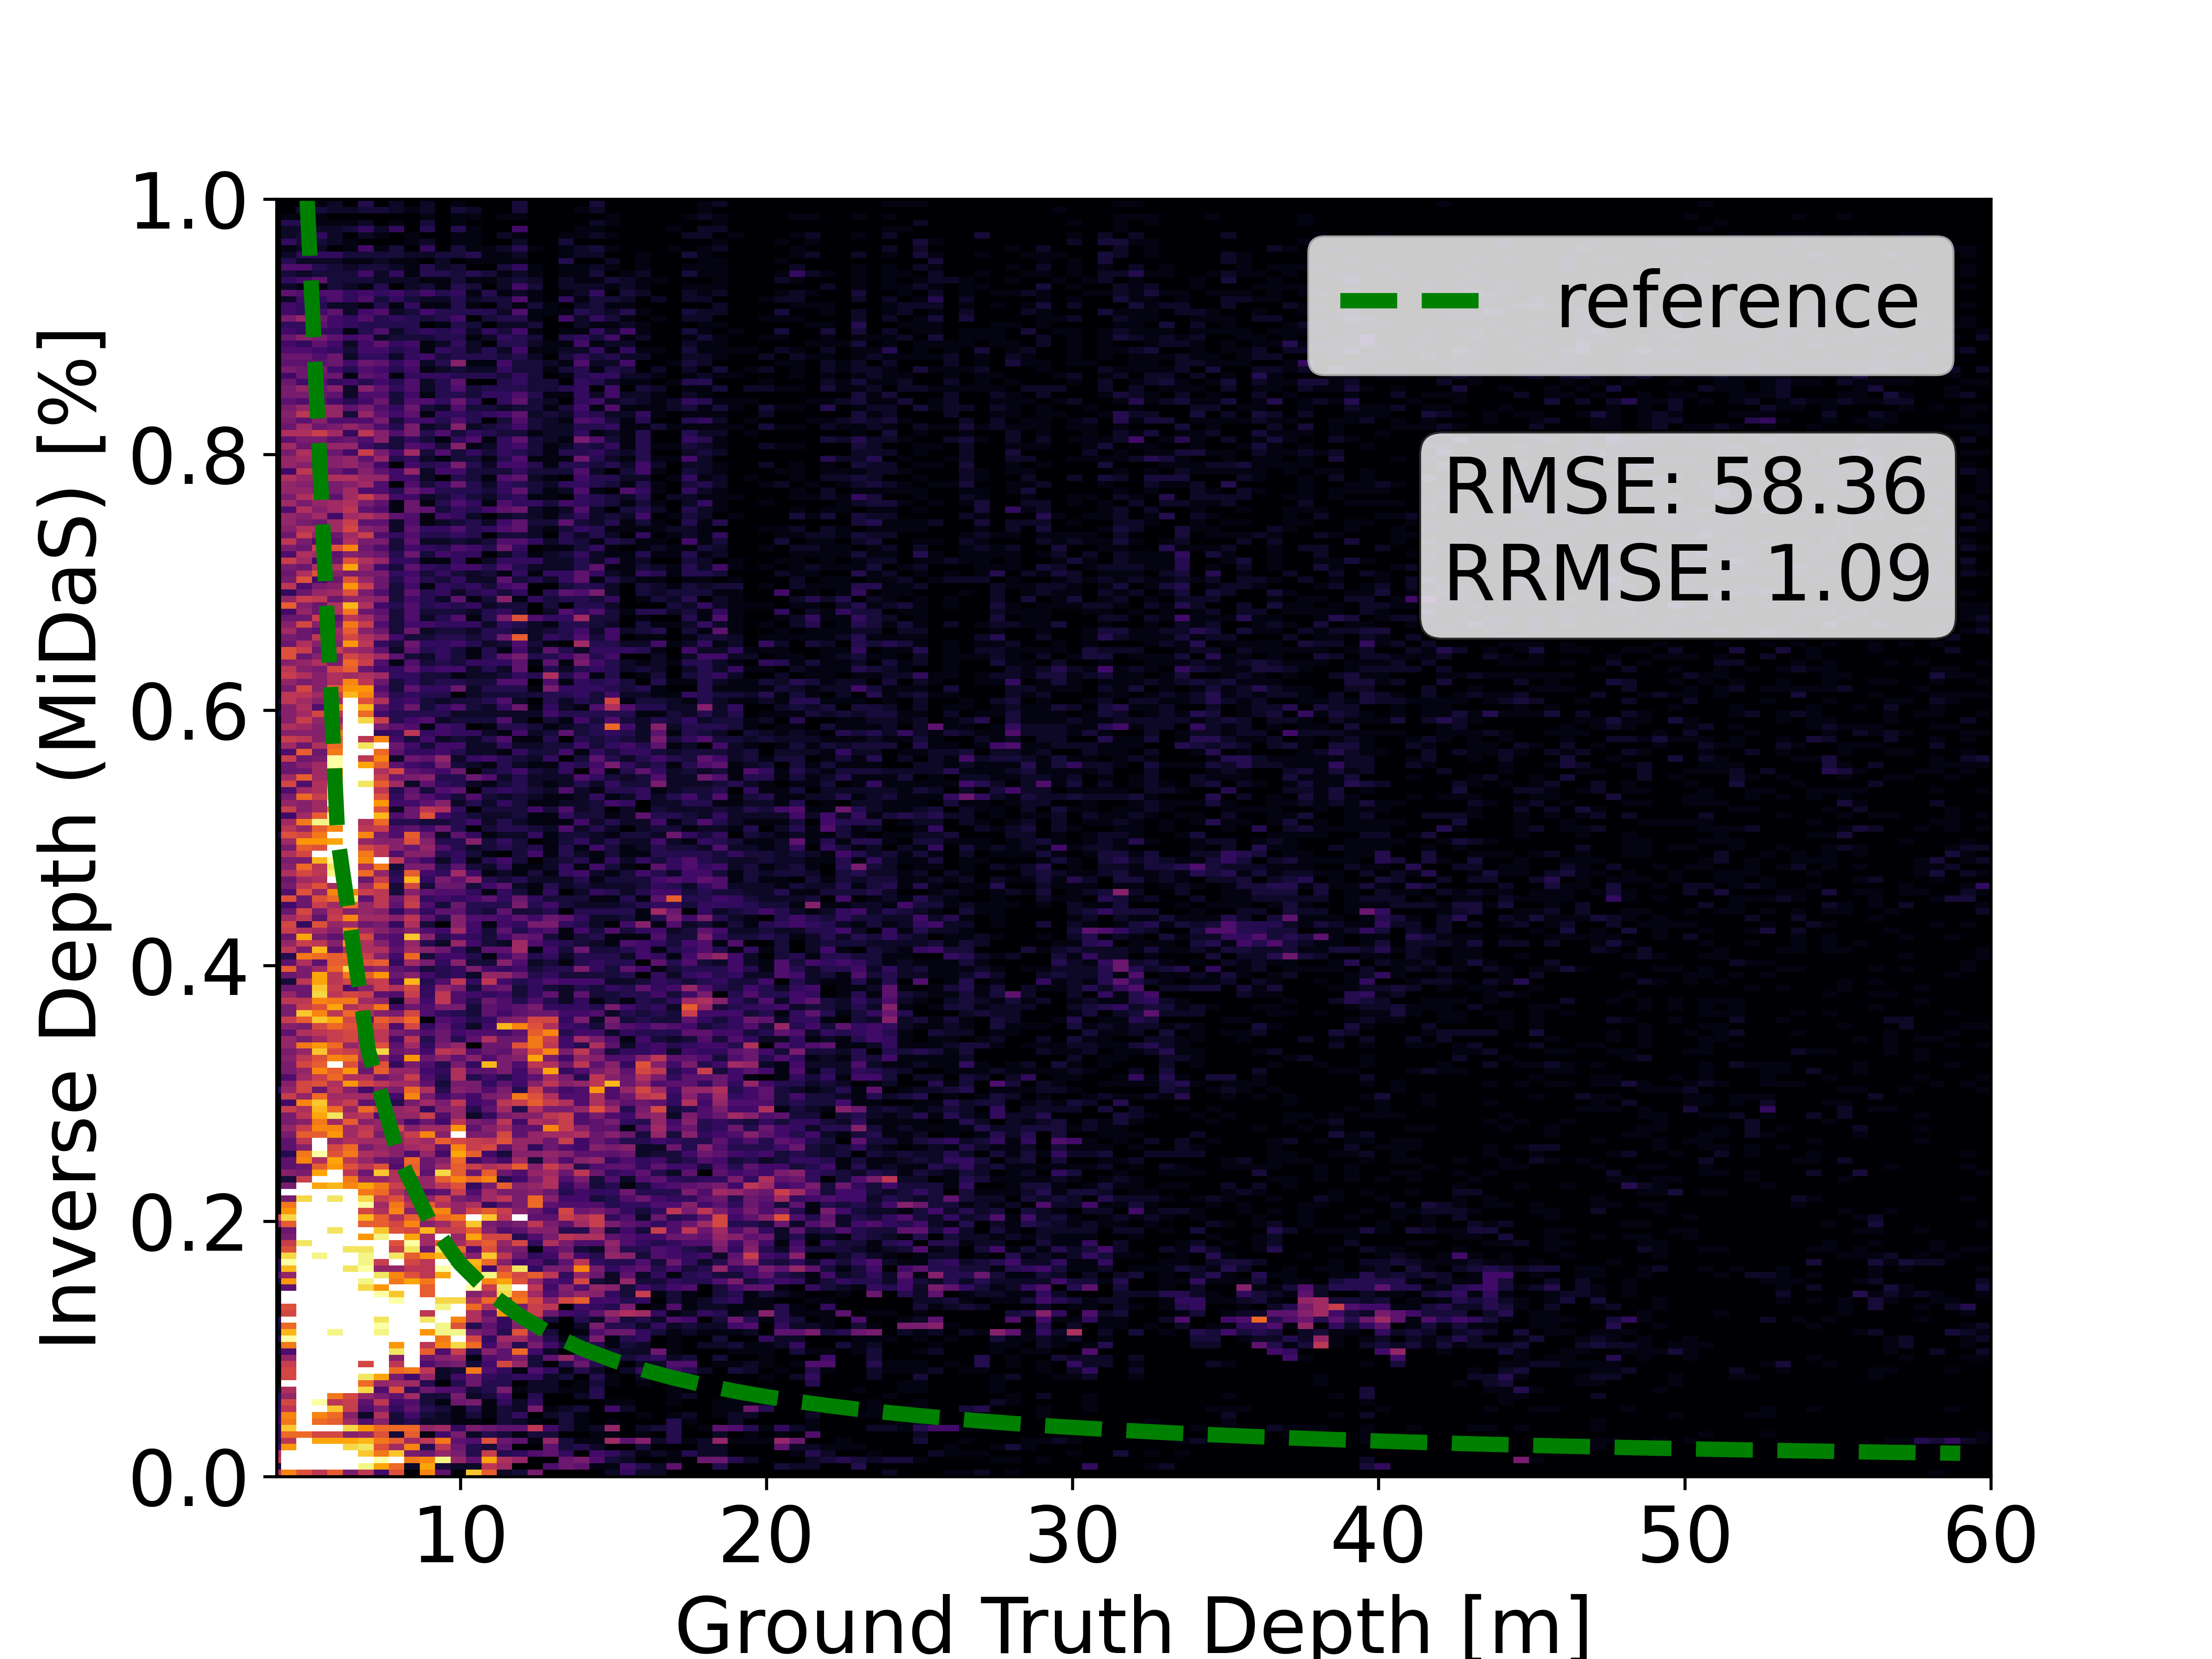
\includegraphics[width=\textwidth]{images/nuscenes/depth_0.png} % first figure itself
    \end{minipage}\hfill
    \begin{minipage}{0.47\textwidth}
        \centering
        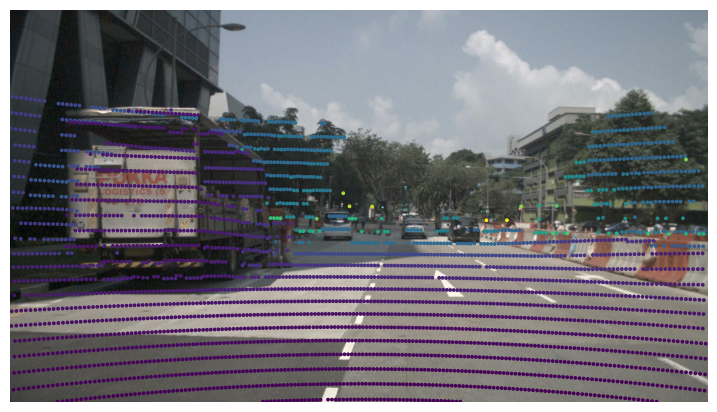
\includegraphics[width=\textwidth, height=4.8cm]{images/nuscenes/lidar_over_img.png} % second figure itself
    \end{minipage}
    \caption{Monocular depth estimation with MiDaS on NuScenes dataset \cite{nuscenes}.
    \textbf{Left}: Relative inverse depth estimated from the model compared to 
    the ground-truth information taken from the front LiDAR for an entire scene.
    \textbf{Right}: Projection of the LiDAR point cloud on the image plane for
    one sample of the same scene.} 
    \label{fig:mde}
\end{figure}



\section {Deep Learning-based Approach}
Sample text
\subsection {Data Distribution of BDD100k}
\subsection{Supervised Training on Dr(eye)ve}
\subsection{Semi-Supervised Training on Dr(eye)ve}
\subsection{Supervised Training on BDD100k}
\subsection{Semi-Supervised Training on BDD100k}

\subsection{Experiments with GPT4-o}
In May 2024, OpenAI released GPT4-o, their multilingual, multimodal generative 
pre-trained transformer. Considering its powerful capability to describe general 
contexts in wide scenes, we decided to test the architecture to solve a problem 
similar to ours. Experiments were conducted on BDD100k dataset.

\subsubsection{Problem Definition}
We defined two groups of six images each. The first group consists of general 
driving scenarios that contain at least one person in each image. 
The second group, on the other hand, is still related to driving scenarios but 
does not contain any person. However, in most images of both groups there are 
some common objects, including cars, buildings, etc.
Then the model will be asked to evaluate a new, never seen, image and answer 
in which group it belongs.

Other experiments in the two groups were done, including asking the model which 
common targets are present in each group.

\subsubsection{Data Selections}
\setlength{\subfigwidth}{45mm}
\setlength{\horspace}{.3\textwidth}
\begin{figure}
    \centering
    \begin{tabular}{p{\horspace} p{\horspace} p{\horspace}}
    \begin{subfigure}[b]{\subfigwidth}
        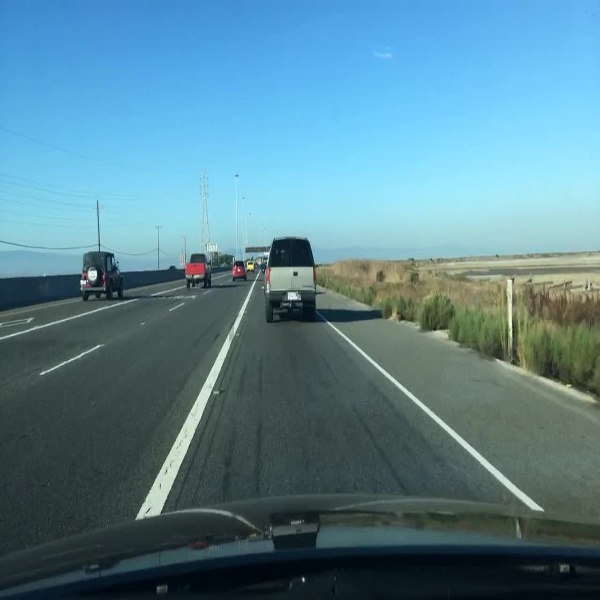
\includegraphics[width=\subfigwidth]{images/gpt4/s1.jpg}
    \end{subfigure}
    \hfill &
    \begin{subfigure}[b]{\subfigwidth}
        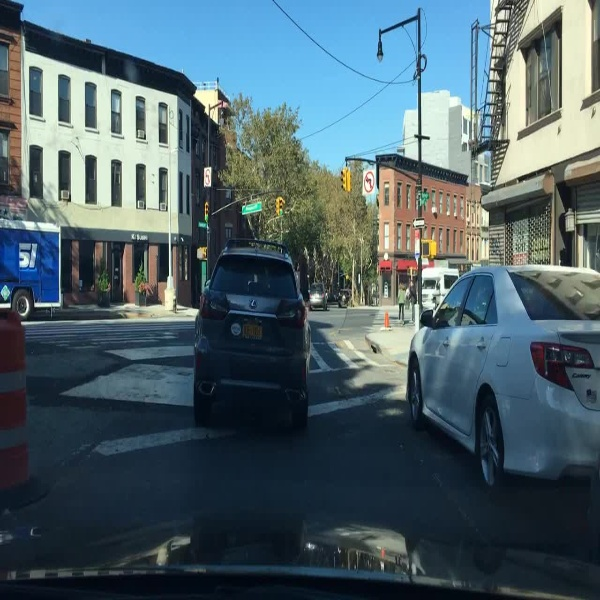
\includegraphics[width=\subfigwidth]{images/gpt4/s2.jpg}
    \end{subfigure} 
    \hfill &
    \begin{subfigure}[b]{\subfigwidth}
        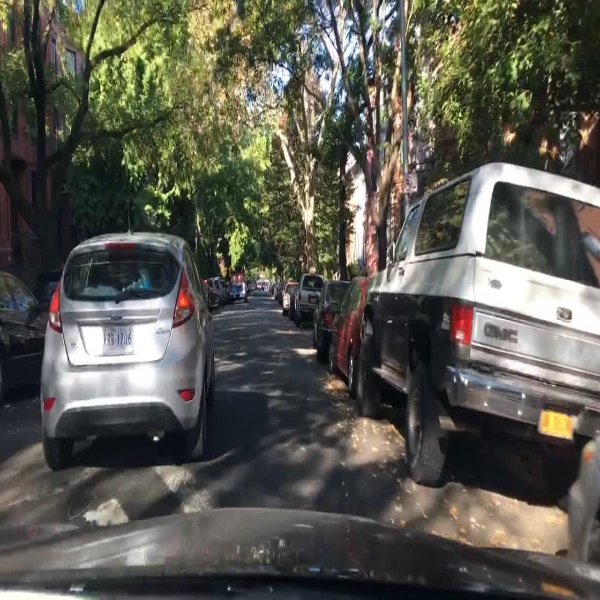
\includegraphics[width=\subfigwidth]{images/gpt4/s3.jpg}
    \end{subfigure} \\
    %
    \begin{subfigure}[b]{\subfigwidth}
        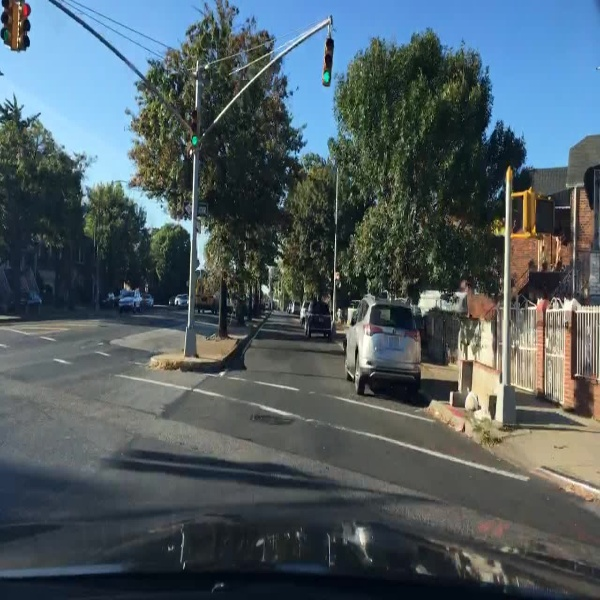
\includegraphics[width=\subfigwidth]{images/gpt4/s4.jpg}
    \end{subfigure}
    \hfill &
    \begin{subfigure}[b]{\subfigwidth}
        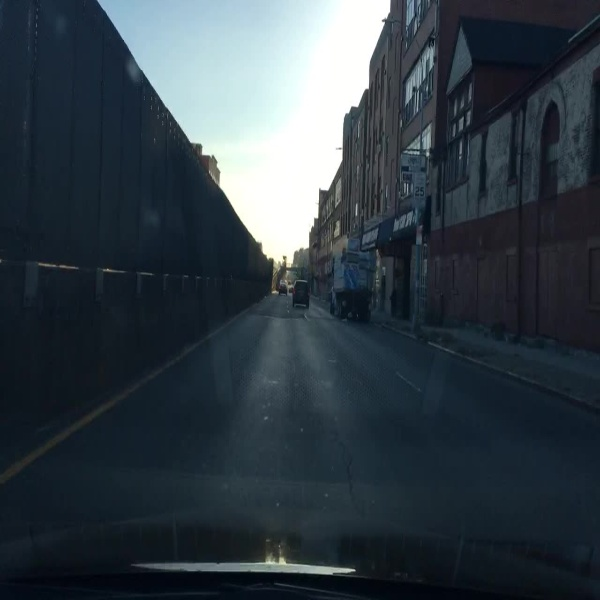
\includegraphics[width=\subfigwidth]{images/gpt4/s5.jpg}
    \end{subfigure} 
    \hfill &
    \begin{subfigure}[b]{\subfigwidth}
        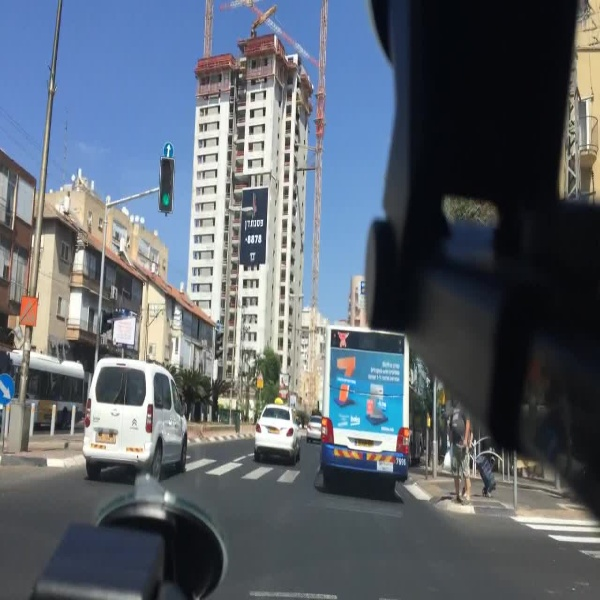
\includegraphics[width=\subfigwidth]{images/gpt4/s6.jpg}
    \end{subfigure}
\end{tabular}
\caption{Group of safe images, there are no people in all the images.}
\label{fig:safe_group}
\end{figure}
%
\begin{figure}
    \centering
    \begin{tabular}{p{\horspace} p{\horspace} p{\horspace}}
    \begin{subfigure}[b]{\subfigwidth}
        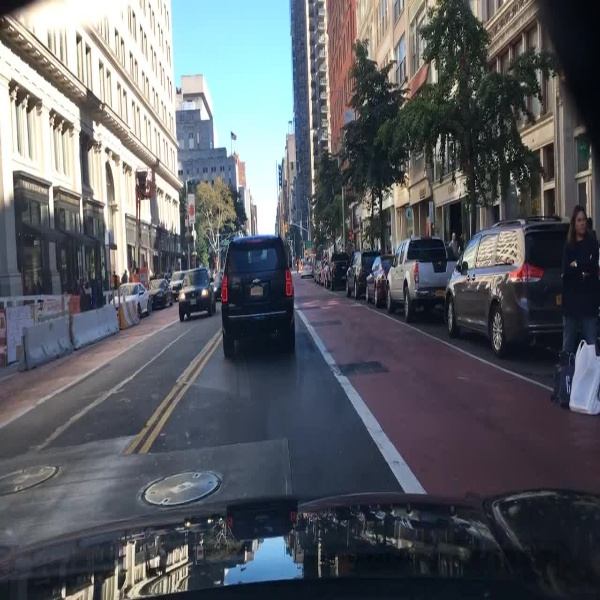
\includegraphics[width=\subfigwidth]{images/gpt4/d1.jpg}
    \end{subfigure}
    \hfill &
    \begin{subfigure}[b]{\subfigwidth}
        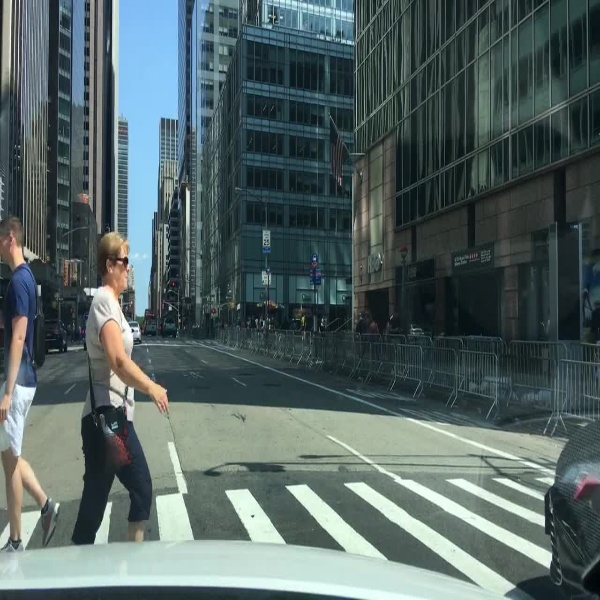
\includegraphics[width=\subfigwidth]{images/gpt4/d2.jpg}
    \end{subfigure} 
    \hfill &
    \begin{subfigure}[b]{\subfigwidth}
        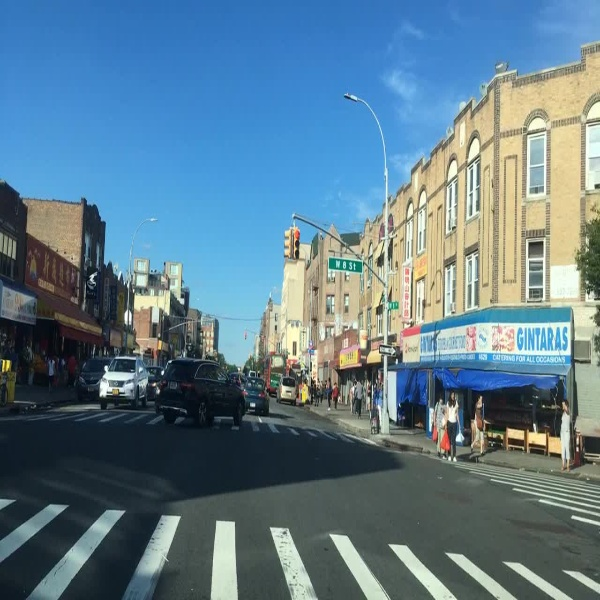
\includegraphics[width=\subfigwidth]{images/gpt4/d3.jpg}
    \end{subfigure} \\
    %
    \begin{subfigure}[b]{\subfigwidth}
        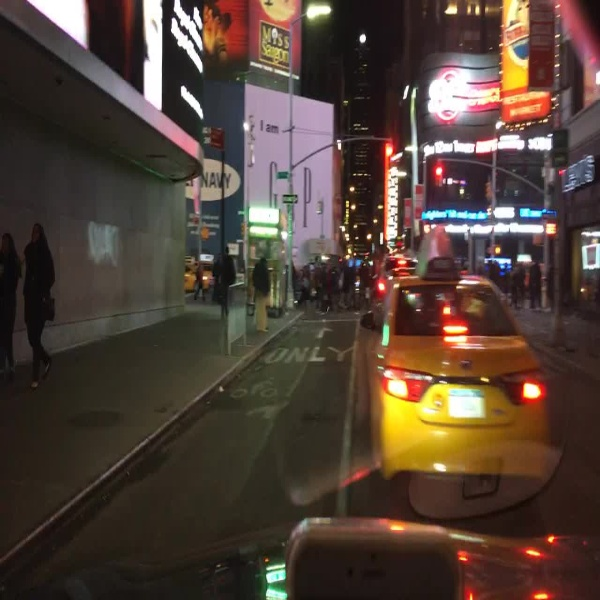
\includegraphics[width=\subfigwidth]{images/gpt4/d4.jpg}
    \end{subfigure}
    \hfill &
    \begin{subfigure}[b]{\subfigwidth}
        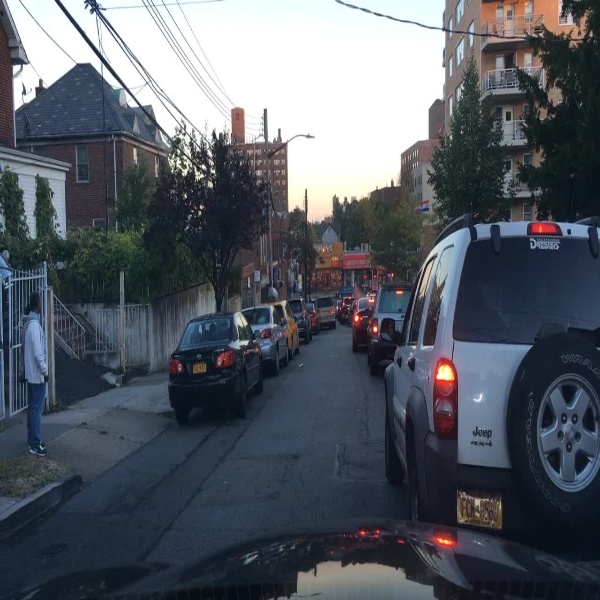
\includegraphics[width=\subfigwidth]{images/gpt4/d5.jpg}
    \end{subfigure} 
    \hfill &
    \begin{subfigure}[b]{\subfigwidth}
        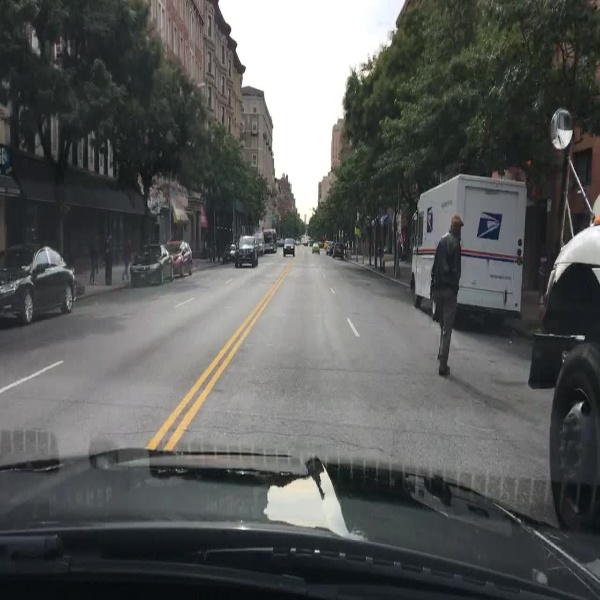
\includegraphics[width=\subfigwidth]{images/gpt4/d6.jpg}
    \end{subfigure}
\end{tabular}
\caption{Group of dangerous images, there are some people in each image.}
\label{fig:dangerous_group}
\end{figure}
The first group of images is shown in Figure \ref{fig:safe_group}. It consists 
of six images that do not contain any person. In particular, in the first image 
on the top left there is the ego-vehicle in a highway with some other vehicles 
on the front. The second on the top-center represents a downtown scenario with 
some vehicles on the front. In the third image on top-right there is a vehicle 
on the front and many vehicles parked on both sides of the road. The fourth 
image on bottom-left represents the ego-vehicle driving on a road with a traffic 
divider and some cars parked on the right side. In the fifth image on the 
bottom-center there is a straight road with some vehicles on the front and tall 
buildings on the sides. The last image on the bottom-right represents a 
downtown scenario with some vehicles, including cars and a bus. There is 
actually an occluded person in the image, but it is almost not visible.

The second group of images is shown in Figure \ref{fig:dangerous_group}. 
In the first image on the top-left there are two cars in fron of the ego-vehicle, 
some cars parked on both sides and a pedestrian standing on the right side. There 
are also some other pedestrians far away on sidewalks, not much visible in the 
image.
The second image on the top-center represents a downtown scenario where some 
pedestrians are crossing the road. There is also a car partially visible on the 
right of the ego-vehicle. The environment is characterized by tall buildings.
The third image on the top-right represents a downtown scenario with some 
empty crosswalks but many pedestrians on sidewalks. There are also some cars 
driving on the main road.
The fourth image on the bottom-left represents a night downtown scenario with a 
taxi in front of the ego-vehicle and group of pedestrians on the left sidewalk 
and far away, where there are crosswalks and red traffic lights.
In the fifth image, bottom-center, there is a line of cars in front of the 
ego-vehicle, some cars parked on the left side, and a pedestrian standing on the 
left sidewalk.
The last image on the bottom-right represents a main road with some vehicles 
parked on both sides, some others driving, and a person standing on the right 
side of the road.

Considering the dangerous scenarios, some specific cases were carefully selected,
especially with people partially visible, in the corners of the images, and 
on the background. On the other hand, in both groups there are many vehicles, both 
in foreground and background, that contribute to add noise to the data to 
classify.
This decision represents a further challenge for the model to 
isolate the right group of pixels.

\subsubsection{Common Features Extraction}
The first experiment consists of showing the model the two groups of images, 
without explicitly explaining the difference between them. The model is asked 
to describe the common targets in each group. The question-answer pairs are 
shown below:
%
{\fontfamily{cmr}\selectfont
\begin{description}
    \item[Q:] What common targets do all the images have?
    Do not list a target if it is not inside all the images. 
    (\emph{showing the dangerous images})
    \item[A:] Cars, roads, \hl{people}, sky.
    \item[Q:] What common targets do all the images have?
    Do not list a target if it is not inside all the images. 
    (\emph{showing the safe images})
    \item[A:] Road, \hl{other vehicles}, sorrounding environment.    
\end{description}
}
It is possible to notice that for the dangerous images the model correctly 
detects also people as common targets. Moreover, vehicles are shown in both 
groups, and the model is able to distinguish them as common targets correctly.
This means that the model is able to extract the common noise in both groups 
(the presence of cars, that usually occupy many pixels with respect to people), 
but at the same time it is able to extract features of people related to the 
dangerous group.

This is a promising result, considering that GPT4 is a pretrained model on 
general multimodal data, and not specifically on driving scenarios. 
However, it has over 174 billion parameters, and that is why it is capable to 
generalize in many different contexts. Using a vision transformer architecture 
for specific tasks, like driving scenarios, with much less parameters, could 
still lead to good results.

\subsubsection{Grouping and Classification}
\setlength{\subfigwidth}{45mm}
\setlength{\horspace}{.3\textwidth}
\begin{figure}
    \centering
    \begin{tabular}{p{\horspace} p{\horspace}}
    \begin{subfigure}[b]{\subfigwidth}
        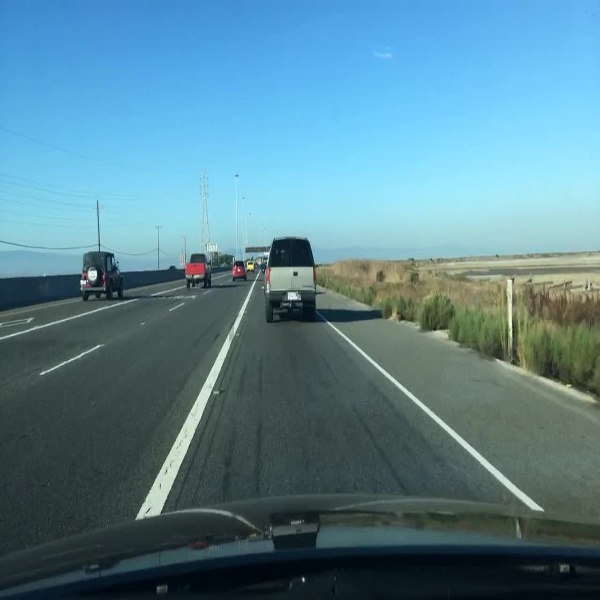
\includegraphics[width=\subfigwidth]{images/gpt4/s1.jpg}
    \end{subfigure}
    \hfill &
    \begin{subfigure}[b]{\subfigwidth}
        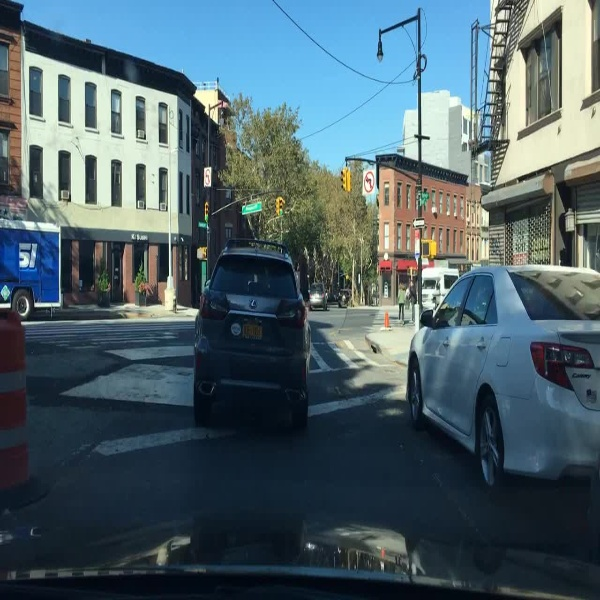
\includegraphics[width=\subfigwidth]{images/gpt4/s2.jpg}
    \end{subfigure} \\
    %
    \begin{subfigure}[b]{\subfigwidth}
        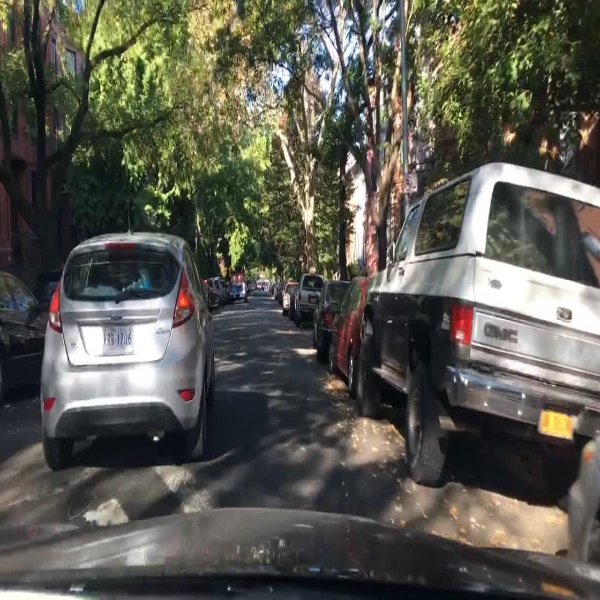
\includegraphics[width=\subfigwidth]{images/gpt4/s3.jpg}
    \end{subfigure}
    \hfill &
    \begin{subfigure}[b]{\subfigwidth}
        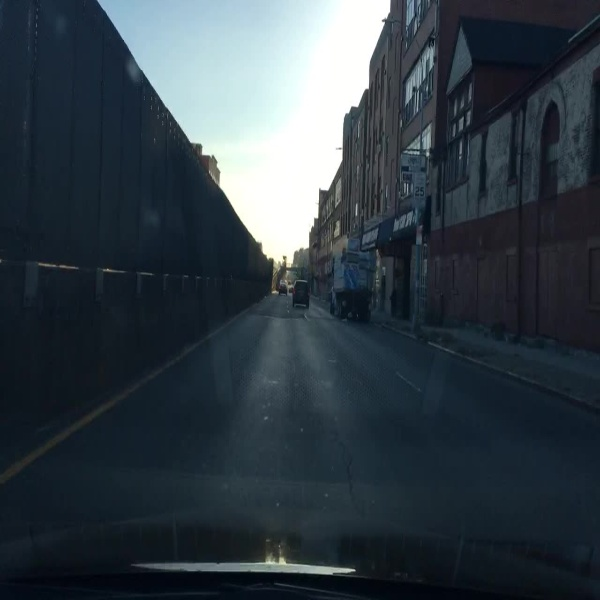
\includegraphics[width=\subfigwidth]{images/gpt4/s5.jpg}
    \end{subfigure}
\end{tabular}
\caption{Group of safe images, there are no people in all the images.}
\label{fig:sub_dangerous_group}
\end{figure}
%
\begin{figure}
    \centering
    \begin{tabular}{p{\horspace} p{\horspace}}
    \begin{subfigure}[b]{\subfigwidth}
        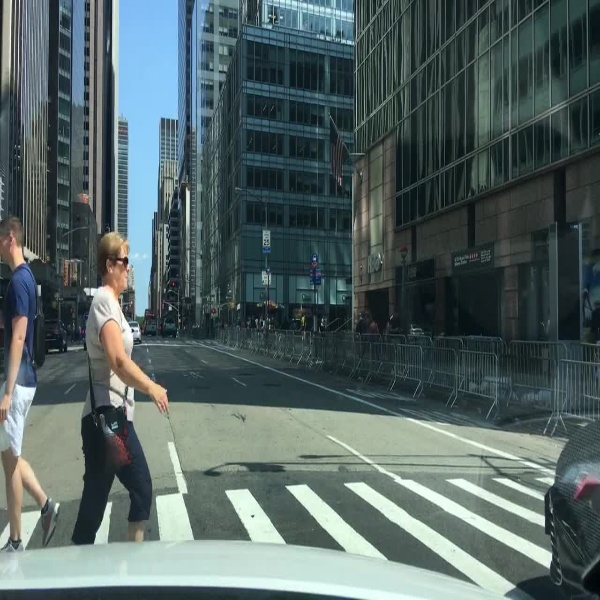
\includegraphics[width=\subfigwidth]{images/gpt4/d2.jpg}
    \end{subfigure}
    \hfill &
    \begin{subfigure}[b]{\subfigwidth}
        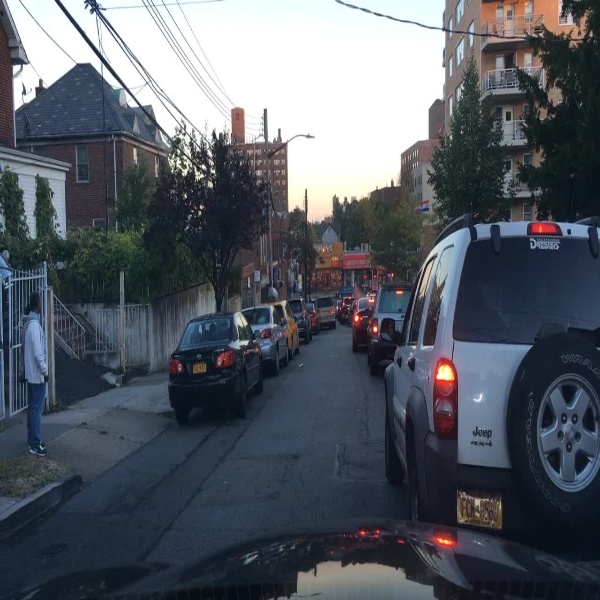
\includegraphics[width=\subfigwidth]{images/gpt4/d5.jpg}
    \end{subfigure} \\
    %
    \begin{subfigure}[b]{\subfigwidth}
        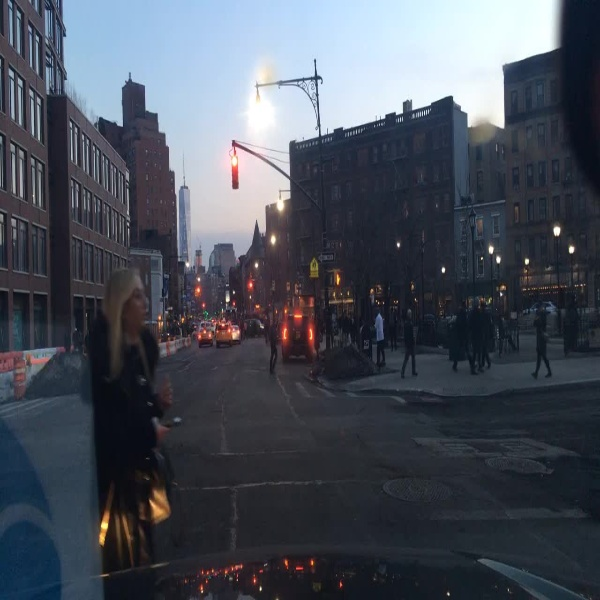
\includegraphics[width=\subfigwidth]{images/gpt4/d7.jpg}
    \end{subfigure}
    \hfill &
    \begin{subfigure}[b]{\subfigwidth}
        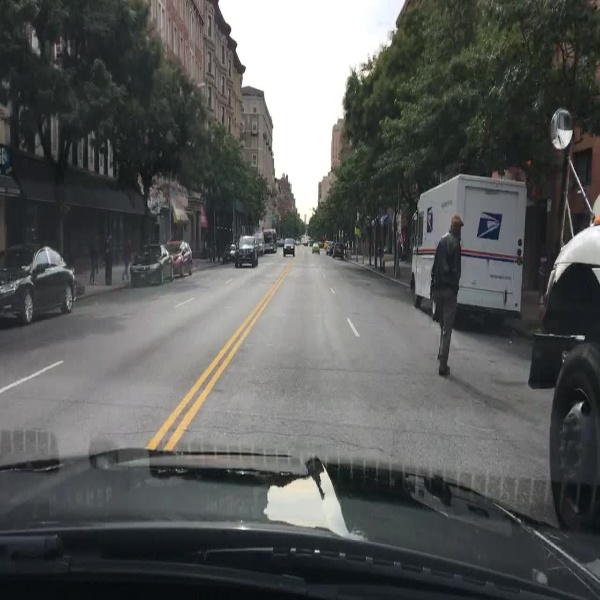
\includegraphics[width=\subfigwidth]{images/gpt4/d6.jpg}
    \end{subfigure}
\end{tabular}
\caption{Group of safe images, there are no people in all the images.}
\label{fig:sub_safe_group}
\end{figure}
\begin{figure}
\centering
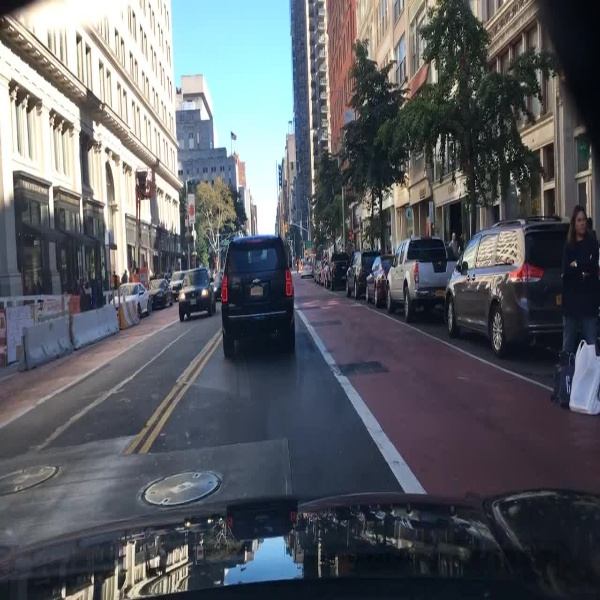
\includegraphics[width=\subfigwidth]{images/gpt4/d1.jpg}
\caption{Test image}
\label{fig:test_image}
\end{figure}

In this experiment we only showed the model the two groups of images, without 
asking to extract common targets. Then we show a new image and ask the model 
to classify it in the right group. The question-answer pairs are shown below:
{\fontfamily{cmr}\selectfont
\begin{description}
    \item[Q:] I will show you two groups of images. Then I will show you a test 
    image and you have to tell me what group it is related to. You have to 
    identify common features for each group to find the correct matching. Do not 
    output anything before I have finished, when I will tell you "predict this 
    image".
    \item[A:] Understood! I'm ready when you are to proceed with the image groups 
    and the test image.
    \item[Q:] This is the first group. (\emph{showing the first group of images})
    \item[A:] I've received the first group of images. Please show me the next group.
    \item[Q:] This is the second group. (\emph{showing the second group of images})
    \item[A:] I've received the second group of images. Please proceed with showing 
    the test image when you are ready.
    \item[Q:] This is the test image. (\emph{showing the test image})
    \item[A:] Based on the test image and comparing it to the two groups shown earlier:
    The test image features an urban setting with buildings lining the streets 
    and multiple vehicles on the road. It closely resembles the environment and 
    context of the images in the second group, which also depict urban settings 
    with buildings, streets, and a 
    \hl{visible presence of pedestrians} or traffic. 
    This environment is distinct from the first group, which primarily showed 
    roads in more open, less densely populated areas or showing less urban 
    characteristics. 
    Therefore, \hl{the test image belongs to the second group}.
\end{description}
}
Also in this experiment the model is able to correctly classify the test image 
in the right group. The model is able to give a detailed explanation of the 
features that are common in the test image and in the second group of images.
It is impressive that the model is capable to give such detailed explanations 
of contexts in images, considering that it is a general model and not specifically 
trained on driving scenarios.
